% vim: tw=80 cc=80
\documentclass[10pt,a4paper,hidelinks]{article}
\usepackage[cm]{fullpage}
\usepackage{hyperref}
\usepackage{caption}
\usepackage{listings}
\usepackage{enumitem}
\usepackage{xcolor}
\usepackage{float}
\usepackage{tikz}
\usetikzlibrary{arrows,automata}

\definecolor{codegreen}{rgb}{0,0.6,0}
\definecolor{codegray}{rgb}{0.5,0.5,0.5}
\definecolor{codepurple}{rgb}{0.58,0,0.82}
\definecolor{backcolour}{rgb}{0.95,0.95,0.95}

\lstdefinestyle{mystyle}{
    backgroundcolor=\color{backcolour},
    commentstyle=\color{codegreen},
    keywordstyle=\color{magenta},
    numberstyle=\tiny\color{codegray},
    stringstyle=\color{codepurple},
    basicstyle=\ttfamily\footnotesize,
    breakatwhitespace=false,
    breaklines=true,
    captionpos=b,
    keepspaces=true,
    numbers=left,
    numbersep=5pt,
    showspaces=false,
    showstringspaces=false,
    showtabs=false,
    tabsize=2,
    frame=single
}

\lstset{style=mystyle}

\setlength{\parindent}{0cm}
\setlength{\parskip}{8pt}

\def\lib{Z80-Retro!-libcpm }

\title{\lib}
\author{David Latham}
\date{September, 2025}


\begin{document}
\maketitle
\tableofcontents
\pagebreak
\section{Introduction}

This guide is intended provide some commentary that can be read along with the
source code to showcase the various components of the library and how they can
be used in your own applications.

You should read the comments in the header files.  They are updated during
development and will be the most accurate.

\subsection{What Is \lib?}

\lib is a C library that you can link to in your applications for
use with the
\href{https://github.com/etchedpixels/fuzix-compiler-kit.git}{FUZIX-Compiler-Kit}.\footnote{https://github.com/etchedpixels/fuzix-compiler-kit.git}
The library is specifically targeted at the
\href{https://github.com/z80-retro}{Z80-Retro!}\footnote{https://github.com/z80-retro} Single Board Computer by John
Winans.

Some standard libraries are implemented where they can be easily backed by the
CP/M 2.2 BDOS function calls.  Additionally the library includes functions for
working with the TMS9918 and Atari style joystick ports on the VDP daughter
board designed for the Z80-Retro!.

For instructions on how to install the compiler and this library, see the
\url{./BUILD.md} documentation.

\subsection{Usage}

You can use the by including the headers you need, calling the functions in
your code and finally compiling and linking. See: "Listing: \ref{lst:makefile}
- Example Makefile" on page \pageref{lst:makefile}

The process is something like this:

\begin{description}[font=$\bullet$~\normalfont\scshape\color{red!50!black}]
  \item[Compile] fcc -O2 -mz80 -Iinclude -I /opt/fcc/lib/z80/include -c -o
    main.o main.c
  \item[Link] ldz80 -b C0x100 -o main.bin crt0.o main.o libcpm.a
  \item[Truncate] dd if=main.bin of=main.com skip=1 bs=256
\end{description}

The linker documentation is very minimal because it's a very minimal linker.
The \texttt{`-b`} switch tells the linker to output a binary file without
relocatable code.  The -C0x100 tells the linker to begin the \texttt{`code`}
segment at 0x100 which is the beginning of the TPA for CP/M.

Because the linker always starts filling code from 0x0000 we need to remove the
first 256 bytes using the \texttt{`dd`} command.
\pagebreak

\begin{center}
  \begin{lstlisting}[caption=Example Makefile]
    TOP=.
    CC=/opt/fcc/bin/fcc
    AS=/opt/fcc/bin/asz80
    LD=/opt/fcc/bin/ldz80

    CFLAGS=-O2 -mz80 -I $(TOP)/../include -I /opt/fcc/lib/z80/include
    LDFLAGS=-b -C0x100
    LIBS=\
         $(TOP)/../libcpm.a \
         /opt/fcc/lib/z80/libz80.a \
         /opt/fcc/lib/z80/libc.a

    CRT=$(TOP)/../crt0.o

    all: clean malloc.com fileio.com testtms.com copy

    malloc.bin: malloc.o
      $(LD) $(LDFLAGS) -o $@ $(CRT) $^ $(LIBS)

    malloc.com: malloc.bin
      dd if=$^ of=$@ skip=1 bs=256

    fileio.bin: fileio.o
      $(LD) $(LDFLAGS) -o $@ $(CRT) $^ $(LIBS)

    fileio.com: fileio.bin
      dd if=$^ of=$@ skip=1 bs=256

    testtms.bin: testtms.o
      $(LD) $(LDFLAGS) -o $@ $(CRT) $^ $(LIBS)

    testtms.com: testtms.bin
      dd if=$^ of=$@ skip=1 bs=256


    clean:
      rm -fv malloc.bin malloc.com fileio.bin fileio.com
      find . -name "*.o" -exec rm -fv {} \;
  \end{lstlisting}
\end{center}
\label{lst:makefile}

This example does not show the actual FCC commands explicitly.  Make is
automating that step for us.
\pagebreak

\section{Headers}

The headers are all located in the projects "include" directory.  You just need
to \texttt{\#include} the ones you need and make sure to link to the
\texttt{libcpm.a} library.

As the code is split out into multiple translation units, your resulting binary
should include almost no wasted code.


\subsection{C Runtime}

There is a provided \texttt{crt0.o} object file which should be included in the
linking stage.  The C runtime performs the following actions:

\begin{description}
  \item[prep stack] Preserve the CP/M stack pointer and set up a new stack
    pointer at the top of the TPA.
  \item[init\_sys] Calls the \texttt{\_init\_sys} routine to initialise the
    "sys\_open\_files" array.
  \item[execute] Call the \texttt{main()} function
  \item[return] Return to CP/M (restoring the CP/M stack and freeing the
    tms\_buffer along the way)
\end{description}

\subsection{tms99xx}

See Graphics Programming on page \pageref{graphicsprogramming} for details.

\subsection{string}

The string library provides basic memory management routines like memset, memcpy
strlen etc.

There is also (in leu of any kind of \texttt{printf} function, to additional
functions for printing text.  Remembering, of course, that CP/M has it's own
BDOS calls for writing text to the terminal.

\subsection{stdlib}

There are two parts to the malloc / free implementation in this library.  The
first is the implementation of the "sbrk()" system call and the second is the
malloc and free functions themselves.

The sbrk() function was copied and adapted from the HiTech C compiler project.

The malloc and free functions are transcribed directly from "The C Programming
Language - Second Edition" By Biran W. Kernignhan and Dennis M. Ritchie.

There are is no defragmentation or garbage collection.  Malloc doesn't usually
make all that much sense in embedded environments.

\begin{description}[font=$\bullet$~\normalfont\scshape\color{red!50!black}]
  \item[abs]
  \item[exit]
  \item[free] From The C Programming Language Book
  \item[itoa]
  \item[malloc] From The C Programming Language Book
  \item[puts] Print a zero terminated string constant to the screen.  No
    formatting.
\end{description}

\subsection{stdio}

\begin{description}[font=$\bullet$~\normalfont\scshape\color{red!50!black}]
  \item[printf] Simple implimentation of \texttt{printf} with support for the
    \%c, \%s, \%d and \%x format specifiers only.
\end{description}

\subsection{cp/m}
The CP/M header provides C wrappers for almost all the CP/M BDOS function calls.

For example, if you want to check for keyboard input without blocking, you can
call the \texttt{cpm\_rawio()} function which returns the ascii char or 0.
Unlike \texttt{cpm\_conin()}, this function does not emit the typed character to
the terminal.

You can find an example of how to use the fileio functions in the "test"
folder.  The "fcntl.h" header file contains lots of additional information.

\break
\section{Graphics Programming} \label{graphicsprogramming}

Figure \ref{fig:gameloop} shows the game loop state machine.  The game state is
initialised before entering the loop.  The loop itself, consists of reading user
input, updating the game state and frame-buffer, waiting for vsync, rendering
the frame-buffer and looping back to user input.

The VSYNC signal from the VDP provides a stable 60 ${\\hertz}$ timer which is
used to normalize game speed on different CPU clock frequencies.  The standard
gameloop waits for the VSYNC signal before rendering to the display to leverage
the fast write cycle times during the vertical blanking interval.

\begin{figure}[H]
  \begin{center}
    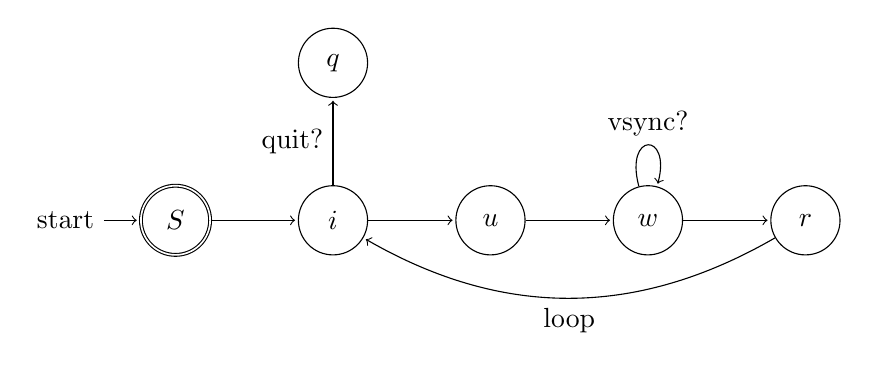
\begin{tikzpicture}[->=stealth',shorten >=1pt,auto,node distance=2cm]
      \node[initial,state,accepting]  (S)               {$S$};
      \node[state]                    (I) [right of=S]  {$i$};
      \node[state]                    (U) [right of=I]  {$u$};
      \node[state]                    (W) [right of=U]  {$w$};
      \node[state]                    (R) [right of=W]  {$r$};
      \node[state]                    (Q) [above of=I]  {$q$};


      \path[->] (S)  edge              node {}      (I)
                (I)  edge              node {}      (U)
                (U)  edge              node {}      (W)
                (W)  edge [loop above] node {vsync?}(W)
                (W)  edge              node {}      (R)
                (R)  edge [bend left]  node {loop}  (I)
                (I)  edge              node {quit?} (Q);
    \end{tikzpicture}
  \end{center}
  \caption{Game Loop}
\label{fig:gameloop}
\end{figure}

There are a range of TMS99xx functions in the \lib to initialise the VDP in the
various display modes and to manage the frame-buffer.

They can be grouped into the following categories:

\begin{description}[font=$\bullet$~\normalfont\scshape\color{red!50!black}]
  \item[Initialization]
    Init the VDP in a display mode, enable interrupts and
    sprite sizes
  \item[Loading data]
    Load patterns, names and colors
  \item[Plotting to the frame buffer]
    Plot tiles or pixels in the XY coordinate
    space into the frame buffer memory.
  \item[Sprites]
    Update sprite attributes to move them around or hide them.
  \item[Flushing the frame buffer to the video memory]
    Stream the framebuffer
    into VDP memory and flush the sprites array into the Sprite Attribute Table in
    VDP memory.
\end{description}


\end{document}
